
%% bare_conf.tex
%% V1.3
%% 2007/01/11
%% by Michael Shell
%% See:
%% http://www.michaelshell.org/
%% for current contact information.
%%
%% This is a skeleton file demonstrating the use of IEEEtran.cls
%% (requires IEEEtran.cls version 1.7 or later) with an IEEE conference paper.
%%
%% Support sites:
%% http://www.michaelshell.org/tex/ieeetran/
%% http://www.ctan.org/tex-archive/macros/latex/contrib/IEEEtran/
%% and
%% http://www.ieee.org/

%%*************************************************************************
%% Legal Notice:
%% This code is offered as-is without any warranty either expressed or
%% implied; without even the implied warranty of MERCHANTABILITY or
%% FITNESS FOR A PARTICULAR PURPOSE! 
%% User assumes all risk.
%% In no event shall IEEE or any contributor to this code be liable for
%% any damages or losses, including, but not limited to, incidental,
%% consequential, or any other damages, resulting from the use or misuse
%% of any information contained here.
%%
%% All comments are the opinions of their respective authors and are not
%% necessarily endorsed by the IEEE.
%%
%% This work is distributed under the LaTeX Project Public License (LPPL)
%% ( http://www.latex-project.org/ ) version 1.3, and may be freely used,
%% distributed and modified. A copy of the LPPL, version 1.3, is included
%% in the base LaTeX documentation of all distributions of LaTeX released
%% 2003/12/01 or later.
%% Retain all contribution notices and credits.
%% ** Modified files should be clearly indicated as such, including  **
%% ** renaming them and changing author support contact information. **
%%
%% File list of work: IEEEtran.cls, IEEEtran_HOWTO.pdf, bare_adv.tex,
%%                    bare_conf.tex, bare_jrnl.tex, bare_jrnl_compsoc.tex
%%*************************************************************************

% *** Authors should verify (and, if needed, correct) their LaTeX system  ***
% *** with the testflow diagnostic prior to trusting their LaTeX platform ***
% *** with production work. IEEE's font choices can trigger bugs that do  ***
% *** not appear when using other class files.                            ***
% The testflow support page is at:
% http://www.michaelshell.org/tex/testflow/



% Note that the a4paper option is mainly intended so that authors in
% countries using A4 can easily print to A4 and see how their papers will
% look in print - the typesetting of the document will not typically be
% affected with changes in paper size (but the bottom and side margins will).
% Use the testflow package mentioned above to verify correct handling of
% both paper sizes by the user's LaTeX system.
%
% Also note that the "draftcls" or "draftclsnofoot", not "draft", option
% should be used if it is desired that the figures are to be displayed in
% draft mode.
%
\documentclass[conference]{IEEEtran}
% Add the compsoc option for Computer Society conferences.
%
% If IEEEtran.cls has not been installed into the LaTeX system files,
% manually specify the path to it like:
% \documentclass[conference]{../sty/IEEEtran}

% Some very useful LaTeX packages include:
% (uncomment the ones you want to load)


% *** MISC UTILITY PACKAGES ***
\usepackage{balance}
\usepackage{ifpdf}
% Heiko Oberdiek's ifpdf.sty is very useful if you need conditional
% compilation based on whether the output is pdf or dvi.
% usage:
% \ifpdf
%   % pdf code
% \else
%   % dvi code
% \fi
% The latest version of ifpdf.sty can be obtained from:
% http://www.ctan.org/tex-archive/macros/latex/contrib/oberdiek/
% Also, note that IEEEtran.cls V1.7 and later provides a builtin
% \ifCLASSINFOpdf conditional that works the same way.
% When switching from latex to pdflatex and vice-versa, the compiler may
% have to be run twice to clear warning/error messages.




% *** CITATION PACKAGES ***
%
%\usepackage{cite}
% cite.sty was written by Donald Arseneau
% V1.6 and later of IEEEtran pre-defines the format of the cite.sty package
% \cite{} output to follow that of IEEE. Loading the cite package will
% result in citation numbers being automatically sorted and properly
% "compressed/ranged". e.g., [1], [9], [2], [7], [5], [6] without using
% cite.sty will become [1], [2], [5]--[7], [9] using cite.sty. cite.sty's
% \cite will automatically add leading space, if needed. Use cite.sty's
% noadjust option (cite.sty V3.8 and later) if you want to turn this off.
% cite.sty is already installed on most LaTeX systems. Be sure and use
% version 4.0 (2003-05-27) and later if using hyperref.sty. cite.sty does
% not currently provide for hyperlinked citations.
% The latest version can be obtained at:
% http://www.ctan.org/tex-archive/macros/latex/contrib/cite/
% The documentation is contained in the cite.sty file itself.




% *** GRAPHICS RELATED PACKAGES ***
%
\ifpdf
  \usepackage[pdftex]{graphicx}
  % declare the path(s) where your graphic files are
  \graphicspath{{../pdf/}{../jpeg/}{img/}}
  % and their extensions so you won't have to specify these with
  % every instance of \includegraph .jpeg,.png}
\else
  % or other class option (dvipsone, dvipdf, if not using dvips). graphicx
  % will default to the driver specified in the system graphics.cfg if no
  % driver is specified.
  \usepackage[dvips]{graphicx}
  % declare the path(s) where your graphic files are
  \graphicspath{{../eps/}}
  % and their extensions so you won't have to specify these with
  % every instance of \includegraphics
  \DeclareGraphicsExtensions{.eps}
\fi% graphicx was written by David Carlisle and Sebastian Rahtz. It is
% required if you want graphics, photos, etc. graphicx.sty is already
% installed on most LaTeX systems. The latest version and documentation can
% be obtained at: 
% http://www.ctan.org/tex-archive/macros/latex/required/graphics/
% Another good source of documentation is "Using Imported Graphics in
% LaTeX2e" by Keith Reckdahl which can be found as epslatex.ps or
% epslatex.pdf at: http://www.ctan.org/tex-archive/info/
%
% latex, and pdflatex in dvi mode, support graphics in encapsulated
% postscript (.eps) format. pdflatex in pdf mode supports graphics
% in .pdf, .jpeg, .png and .mps (metapost) formats. Users should ensure
% that all non-photo figures use a vector format (.eps, .pdf, .mps) and
% not a bitmapped formats (.jpeg, .png). IEEE frowns on bitmapped formats
% which can result in "jaggedy"/blurry rendering of lines and letters as
% well as large increases in file sizes.
%
% You can find documentation about the pdfTeX application at:
% http://www.tug.org/applications/pdftex


% *** MATH PACKAGES ***
%
\usepackage[cmex10]{amsmath}
% A popular package from the American Mathematical Society that provides
% many useful and powerful commands for dealing with mathematics. If using
% it, be sure to load this package with the cmex10 option to ensure that
% only type 1 fonts will utilized at all point sizes. Without this option,
% it is possible that some math symbols, particularly those within
% footnotes, will be rendered in bitmap form which will result in a
% document that can not be IEEE Xplore compliant!
%
% Also, note that the amsmath package sets \interdisplaylinepenalty to 10000
% thus preventing page breaks from occurring within multiline equations. Use:
\interdisplaylinepenalty=2500
% after loading amsmath to restore such page breaks as IEEEtran.cls normally
% does. amsmath.sty is already installed on most LaTeX systems. The latest
% version and documentation can be obtained at:
% http://www.ctan.org/tex-archive/macros/latex/required/amslatex/math/



% *** SPECIALIZED LIST PACKAGES ***
%
%\usepackage{algorithmic}
% algorithmic.sty was written by Peter Williams and Rogerio Brito.
% This package provides an algorithmic environment fo describing algorithms.
% You can use the algorithmic environment in-text or within a figure
% environment to provide for a floating algorithm. Do NOT use the algorithm
% floating environment provided by algorithm.sty (by the same authors) or
% algorithm2e.sty (by Christophe Fiorio) as IEEE does not use dedicated
% algorithm float types and packages that provide these will not provide
% correct IEEE style captions. The latest version and documentation of
% algorithmic.sty can be obtained at:
% http://www.ctan.org/tex-archive/macros/latex/contrib/algorithms/
% There is also a support site at:
% http://algorithms.berlios.de/index.html
% Also of interest may be the (relatively newer and more customizable)
% algorithmicx.sty package by Szasz Janos:
% http://www.ctan.org/tex-archive/macros/latex/contrib/algorithmicx/




% *** ALIGNMENT PACKAGES ***
%
%\usepackage{array}
% Frank Mittelbach's and David Carlisle's array.sty patches and improves
% the standard LaTeX2e array and tabular environments to provide better
% appearance and additional user controls. As the default LaTeX2e table
% generation code is lacking to the point of almost being broken with
% respect to the quality of the end results, all users are strongly
% advised to use an enhanced (at the very least that provided by array.sty)
% set of table tools. array.sty is already installed on most systems. The
% latest version and documentation can be obtained at:
% http://www.ctan.org/tex-archive/macros/latex/required/tools/


\usepackage{mdwmath}
\usepackage{mdwtab}
% Also highly recommended is Mark Wooding's extremely powerful MDW tools,
% especially mdwmath.sty and mdwtab.sty which are used to format equations
% and tables, respectively. The MDWtools set is already installed on most
% LaTeX systems. The lastest version and documentation is available at:
% http://www.ctan.org/tex-archive/macros/latex/contrib/mdwtools/


% IEEEtran contains the IEEEeqnarray family of commands that can be used to
% generate multiline equations as well as matrices, tables, etc., of high
% quality.


%\usepackage{eqparbox}
% Also of notable interest is Scott Pakin's eqparbox package for creating
% (automatically sized) equal width boxes - aka "natural width parboxes".
% Available at:
% http://www.ctan.org/tex-archive/macros/latex/contrib/eqparbox/





% *** SUBFIGURE PACKAGES ***
%\usepackage[tight,footnotesize]{subfigure}
% subfigure.sty was written by Steven Douglas Cochran. This package makes it
% easy to put subfigures in your figures. e.g., "Figure 1a and 1b". For IEEE
% work, it is a good idea to load it with the tight package option to reduce
% the amount of white space around the subfigures. subfigure.sty is already
% installed on most LaTeX systems. The latest version and documentation can
% be obtained at:
% http://www.ctan.org/tex-archive/obsolete/macros/latex/contrib/subfigure/
% subfigure.sty has been superceeded by subfig.sty.



%\usepackage[caption=false]{caption}
%\usepackage[font=footnotesize]{subfig}
% subfig.sty, also written by Steven Douglas Cochran, is the modern
% replacement for subfigure.sty. However, subfig.sty requires and
% automatically loads Axel Sommerfeldt's caption.sty which will override
% IEEEtran.cls handling of captions and this will result in nonIEEE style
% figure/table captions. To prevent this problem, be sure and preload
% caption.sty with its "caption=false" package option. This is will preserve
% IEEEtran.cls handing of captions. Version 1.3 (2005/06/28) and later 
% (recommended due to many improvements over 1.2) of subfig.sty supports
% the caption=false option directly:
\usepackage[caption=false,font=footnotesize]{subfig}
%
% The latest version and documentation can be obtained at:
% http://www.ctan.org/tex-archive/macros/latex/contrib/subfig/
% The latest version and documentation of caption.sty can be obtained at:
% http://www.ctan.org/tex-archive/macros/latex/contrib/caption/




% *** FLOAT PACKAGES ***
%
%\usepackage{fixltx2e}
% fixltx2e, the successor to the earlier fix2col.sty, was written by
% Frank Mittelbach and David Carlisle. This package corrects a few problems
% in the LaTeX2e kernel, the most notable of which is that in current
% LaTeX2e releases, the ordering of single and double column floats is not
% guaranteed to be preserved. Thus, an unpatched LaTeX2e can allow a
% single column figure to be placed prior to an earlier double column
% figure. The latest version and documentation can be found at:
% http://www.ctan.org/tex-archive/macros/latex/base/



%\usepackage{stfloats}
% stfloats.sty was written by Sigitas Tolusis. This package gives LaTeX2e
% the ability to do double column floats at the bottom of the page as well
% as the top. (e.g., "\begin{figure*}[!b]" is not normally possible in
% LaTeX2e). It also provides a command:
%\fnbelowfloat
% to enable the placement of footnotes below bottom floats (the standard
% LaTeX2e kernel puts them above bottom floats). This is an invasive package
% which rewrites many portions of the LaTeX2e float routines. It may not work
% with other packages that modify the LaTeX2e float routines. The latest
% version and documentation can be obtained at:
% http://www.ctan.org/tex-archive/macros/latex/contrib/sttools/
% Documentation is contained in the stfloats.sty comments as well as in the
% presfull.pdf file. Do not use the stfloats baselinefloat ability as IEEE
% does not allow \baselineskip to stretch. Authors submitting work to the
% IEEE should note that IEEE rarely uses double column equations and
% that authors should try to avoid such use. Do not be tempted to use the
% cuted.sty or midfloat.sty packages (also by Sigitas Tolusis) as IEEE does
% not format its papers in such ways.





% *** PDF, URL AND HYPERLINK PACKAGES ***
%
\usepackage[hyphens]{url}
% url.sty was written by Donald Arseneau. It provides better support for
% handling and breaking URLs. url.sty is already installed on most LaTeX
% systems. The latest version can be obtained at:
% http://www.ctan.org/tex-archive/macros/latex/contrib/misc/
% Read the url.sty source comments for usage information. Basically,
% \url{my_url_here}.





% *** Do not adjust lengths that control margins, column widths, etc. ***
% *** Do not use packages that alter fonts (such as pslatex).         ***
% There should be no need to do such things with IEEEtran.cls V1.6 and later.
% (Unless specifically asked to do so by the journal or conference you plan
% to submit to, of course. )


% correct bad hyphenation here
\hyphenation{op-tical net-works semi-conduc-tor}

%%%%%%%%%%%%%%%%%%%%%%%%%%%%%%%%%%%
% BOLSTER PACKAGES FOR DEV PERIOD %
%%%%%%%%%%%%%%%%%%%%%%%%%%%%%%%%%%%

\usepackage{booktabs, multirow}
\usepackage{amssymb}
%\usepackage{hyperref}
\usepackage{tabularx}
\graphicspath{{../../../Figures/}{./figures/}}

\begin{document}
\IEEEoverridecommandlockouts
%\IEEEpubid{978-1-5090-2696-8/16/\$31.00 \copyright 2016 IEEE}
\IEEEpubid{\makebox[\columnwidth]{\hfill 978-1-5090-2696-8/16/\$31.00~\copyright~2016~IEEE} \hspace{\columnsep}\makebox[\columnwidth]{ }}
\IEEEpubidadjcol

% paper title
% can use linebreaks \\ within to get better formatting as desired
\title{Analytical Metric Weight Generation for Multi-Domain Trust in Autonomous Underwater MANETs}


% author names and affiliations
% use a multiple column layout for up to three different
% affiliations
\author{\IEEEauthorblockN{Andrew Bolster, Alan Marshall}
\IEEEauthorblockA{Department of Electrical Engineering and Electronics\\
University of Liverpool\\
Liverpool, UK\\
Email: {andrew.bolster,alan.marshall}@liverpool.ac.uk}
}% use for special paper notices
\IEEEspecialpapernotice{(Invited Paper)}

% make the title area
\maketitle

\begin{abstract}
%\boldmath

Trust Management Frameworks (TMFs) are being used to improve the efficiency, security, and reliability of decentralized and distributed autonomous MANETs using metrics garnered from the communications activities of nodes within the networks.
However, these do not perform well in sparse / harsh environments such as those found in Underwater Acoustic Networks (UANs)~\cite{Bolster2015}.
As node capabilities increase, the physical motion of nodes represent an additional domain of knowledge about the operations and behaviours of the network.

In this paper we present a Machine Learning supported methodology for optimising metric weight vector generation, using metrics from both physical and communications domains to detect and identify a range of misbehaviours, demonstrating that by utilising information from multiple domains, trust assessment can be more sensitive and accurate than in single-domain (communications) assessment.
\end{abstract}
% no keywords

% For peer review papers, you can put extra information on the cover
% page as needed:
% \ifCLASSOPTIONpeerreview
% \begin{center} \bfseries EDICS Category: 3-BBND \end{center}
% \fi
%
% For peerreview papers, this IEEEtran command inserts a page break and
% creates the second title. It will be ignored for other modes.
\IEEEpeerreviewmaketitle



\section{Introduction}
% no \IEEEPARstart
\IEEEpubidadjcol

Trust Management Frameworks (TMFs) in terrestrial MANETs has been an area of active research for many years; with implicitly limited resources in terms of power, mobility, and communications range, the elimination or isolation of malicious nodes within the MANET is an obvious method for maintaining performance and security. 
TMFs provide information to assist the estimation of future states and actions of nodes within networks. 
This information is used to optimise the performance of a network against malicious, selfish or defective misbehaviour by one or more nodes. 
Existing research has demonstrated the advantages of implementing TMFs to 802.11 based MANETs in terms of preventing selfish operation and maintinaing throughput in the presence of malicious nodes \cite{Li2007,Buchegger2002}.
However, as these decentralised networks expand beyond the terrestrial arena into aerial and underwater environments, these Trust frameworks must be assessed for their suitability to these new regions of operation.

With respect to the comparatively stable terrestrial RF environment, the underwater acoustic communications environment is unforgiving; generally static or stable assumptions about propagation delay and paths, frequency-based attenuation and minimal refraction simply don't apply to many marine communications channels.
This, coupled with the highly location, depth, weather, and flora and fauna dependent variability of these fundamental channel parameters make it difficult to make assume that instantenous or short-channel fading are the result of a misbehaving node or of a whale passing between nodes.

In this paper we build upon previous work \cite{Bolster2015} that demonstrated the use of  Random Forest regression \cite{Breiman2001} to assess the relative importance of Communications Metrics in a simulated UAN, and extend the presented methodology with novel optimisation target functions and applying these methods of Metric Assessment across both Physical and Communications metric domains against both communications and physical misbehaviours.
This physical metric assessment uses the motion of nodes within a team to detect and potentially identify malicious or failing operation within a cohort.
This is accomplished by looking specifically at operations within the three dimensions of the underwater space, based on kinematics of industry standard AUVs, the REMUS 100.

This paper is laid out as follows: Sec.~\ref{sec:mtfm} outlines the operation and parameters of the Multi-parameter Trust Framework for MANETs (MTFM) and summarises the comparison of MTFM and other terrestrial MANET TMFs in a simulated marine environment.
Sec.~\ref{sec:weight_ass} discusses the proposed weight generation and assessment scheme for Multi-Domain MTFM, presents the experimental scenarios used, and the analysis method applied.
The results of this analysis are discussed in Sec.~\ref{sec:results}.

\section{Trust for Marine Communication}\label{sec:mtfm}

\subsection{Terrestrial Trust Management Frameworks}

\subsubsection{Single Metric TMFs}

Single Metric TMFs such as Hermes~\cite{Zouridaki2005}, Objective Trust Management Framework (OTMF)~\cite{Li2008} and CONFIDANT~\cite{Buchegger2002} can be generalised as single-value estimation based on a binary input state (success or failure of packet delivery); generating a probabilistic estimation of the future states of that input. 

These single metric TMFs provide malicious actors with a significant advantage if their activity does not impact that metric.
In the case where the attacker can subvert the TMF, the metric under assessment by that TMF does not cover the threat mounted by the attacker.
An example of such a situation would be in a TMF focused on Packet Loss Rate (PLR) where an attacker selectively delays packets going through it, reducing overall throughput but not dropping any packets.
Such behaviour would not be detected by the TMF.

\subsubsection{Multi-parameter Trust for MANETs (MTFM)}

Guo et al. \cite{Guo11} demonstrated the ability of grey relational analysis (GRA) \cite{Zuo1995} to normalise and combine disparate traits of a communications link such as instantaneous throughput, received signal strength, etc. into a grey relational coefficient (GRC), or a ``trust vector'' in this instance.
MTFM performs cohort based normalization of metrics at runtime, providing a grey ``grade'' of trust compared to other observed nodes in that interval, while maintaining the ability to abstract trust values for decision support without requiring per-environment calibration or characterisation.
These assessments are relative in both fairly and unfairly operating networks; all nodes receive mid-range trust assessments if there are no malicious actors as there is nothing ``bad'' to compare against, and variations in assessment will be primarily driven by topological and environmental factors.

The grey relational vector is given as
%
\begin{align}
  \label{eq:grc}
  \theta_{k,j}^t = \frac{\min_k|a_{k,j}^t - g_j^t| + \rho \max_k|a_{k,j}^t-g_j^t|}{|a_{k,j}^t-g_j^t| + \rho \max_k|a_{k,j}^t-g_j^t|} \\
  \phi_{k,j}^t = \frac{\min_k|a_{k,j}^t - b_j^t| + \rho \max_k|a_{k,j}^t-b_j^t|}{|a_{k,j}^t-b_j^t| + \rho \max_k|a_{k,j}^t-b_j^t|} \notag 
\end{align}
%
where $a_{k,j}^t$ is the value of an observed metric $x_j$ for a given node $k$ at time $t$, $\rho$ is a distinguishing coefficient set to $0.5$, $g$ and $b$ are respectively the ``good'' and ``bad'' reference metric sequences from $\{a_{k,j}^t k=1,2\dots K\}$, i.e. $g_j=\max_k({a_{k,j}^t})$,  $b_j=\min_k({a_{k,j}^t})$ (where each metric is selected to be monotonically positive for trust assessment, e.g. higher throughput is presumed to be always better. The implications of this are discussed in Sec.~\ref{sec:weight_ass}). 

This Grey Vector is weighted on a per-metric basis~\eqref{eq:metric_weighting} to then generate a scalar trust value~\eqref{eq:scalarised}. 
%
\begin{align}
  [\theta_k^t, \phi_k^t] &= \left[\sum_{j=0}^M h_j \theta_{k,j}^t,\sum_{j=0}^M h_j \phi_{k,j}^t \right] \label{eq:metric_weighting}\\
  T_k^t &= ({1+{(\phi_k^t)^2}/{(\theta_k^t)^2}})^{-1} \label{eq:scalarised}
\end{align}
%
Where $H=[h_0\dots h_M]$ is a metric weighting vector such that $\sum h_j = 1$, and in unweighted case, $H=[\frac{1}{M},\frac{1}{M}\dots\frac{1}{M}]$.
$\theta$ and $\phi$ are then scaled to $[0,1]$ using the mapping $y = 1.5 x - 0.5$.
To minimise the uncertainties of belonging to either best ($g$) or worst ($b$) sequences in \eqref{eq:grc} the $[\theta,\phi]$ values are reduced into a scalar trust value by\eqref{eq:scalarised}\cite{Hong2010}.
MTFM combines this GRC with a topology-aware weighting scheme and a fuzzy whitenization model, however the model parameter we are primarily interested in is the weighting of metrics for MTFM, which enables the detection and identification of misbehaviours.

\subsection{Summary of Previous Work}
In \cite{Bolster2015}, MTFM was compared against Hermes and OTMF in a series of simulated UANs. 
This was framed against a similar comparison applied to validate the development of MTFM~\cite{Guo2012} in terrestrial applications, and as such required rate and range scaling for application to the simulated underwater channel.

This comparison demonstrated that while the performance of MTFM, Hermes and OTMF were all severely reduced in the marine environment, Unweighted MTFM showed a consistent if small (~10\%) deviation in misbehaviour-cases and no such deviation in the Fair case.
When the individual metrics in MTFM were preferentially weighted, it was demonstrated that a ``Relevance Signature'' could be generated for detectable behaviours based on a Random Forest regression of multiple weighted assessments, producing weighting vectors to maximally detect and identify the operation of those misbehaviours.

\section{Weight assessment schemes for MTFM}\label{sec:weight_ass}

From \eqref{eq:metric_weighting}, the final trust assessment value arrived at are dependent on metric values, the weights assigned to each metric, and the structure of the $g$, $b$ comparison vectors.
The construction of the $g$ and $b$ vectors from~\ref{eq:grc} depends on the trustworthiness-correlations of a particular metric, e.g. Throughput is assumed to be positively correlated to trustworthiness and so follows the basic construction ($g \mapsto \max, b \mapsto \min$).
However, in the case of a metric such as delay, this relationship is inverted; longer delays indicate less trustworthy activity.
In complex environments, the relationship between a metrics trustworthiness correlation may not be quite so obvious as the throughput / delay examples.
This was recognised by Guo, but this ``emphasis/correlation'' weighting was manually configured for each metric for each behaviour and no quantative method for establishing such relationships had been presented since.

We proposed a purely computational methodology for weight generation using a Random Forest Regression and successfully applied it to the communications domain~\cite{Bolster2015}.
We now apply and extend this method to the joint physical-communications metric space.

It is important to establish what analytical behaviour is being targeted; in this case this target is the identifiable exposure of a ``low'' trust value for a misbehaving node that is as distinct from other ``fair'' nodes as possible across a full (or multiple) simulation runs of a particular behaviour given a particular weight vector.
We characterise this ``objective function'' as $\Delta T_{ix}$~\eqref{eq:delta_t}

\begin{align}
  \Delta T_{ix} &= \frac{\sum_{j\neq x}\left( \overline{T_{i,j}}^{\forall t}\right)}{N-1} - \overline{T_{i,x}}^{\forall t} \label{eq:delta_t}\\
\end{align}

Where $i$ is a given observer, $x$ is the suspected misbehaving node, $\overline{T_{i,j}}^{\forall t}$ is the average weighted trust assessment from~\eqref{eq:scalarised} of node $j$ observed by node $i$ across time and $N$ is the number of nodes in the current cohort.

Conceptually, $\Delta T_{ix}$ is the ``Distrust'' of the target node $x$, as the difference in trust value from $0\to1$, the higher the better for our purpose. 
As such, we aim to maximise $\Delta T_{ix}\forall i\neq x$.


\subsection{Available Domain Metrics}

\subsubsection{Communications Metrics}

We use the same trust metrics from \cite{Guo2012} that are applicable to the marine environment, i.e. Delay, Received and Transmitted power, Throughput ($S$), Offered Load ($G$), and Packet Loss Rate (PLR).
Thus, the metric vector for communications-trust assessment is;

\begin{equation}
  X_{comms}=\{D, P_{RX}, P_{TX}, S, G, PLR\}
	\label{eq:comms_vector}
\end{equation}

\subsubsection{Physical Metrics}

Three physical metrics are selected to encompass the relative distributions and activities of nodes within the network; Inter-Node Distance Deviation (INDD), Inter-Node Heading Deviation (INHD), and Node Speed. These metrics encapsulate the relative distributions of position and velocity within the fleet, optimising for the detection of outlying or deviant behaviour within the fleet.

Conceptually, INDD is a measure of the average spacing of an observed node with respect to its neighbours. INHD is a similar approach with respect to node orientation.

\begin{align}
	INDD_{i,j} &= \frac{|P_j - \sum_x \frac{P_x}{N}|}{\frac{1}{N}\sum_x \sum_y{|P_x - P_y| (\forall x \neq y)}}\\
	INHD_{i,j} &= \hat{v} \vert v= V_j - \sum_x{\frac{V_x}{N}}\\
	V_{i,j} &= |V_j|
\end{align}

Thus, the metric vector for physical-trust assessment is;

\begin{equation}
  X_{phy}=\{\text{INDD}, \text{INHD}, V\}
	\label{eq:phys:vector}
\end{equation}

\subsubsection{Cross Domain Trust Metrics}
This simplest possible combination is a vector concatenation across domain metric vectors; 

\begin{align}
  X_{merge} &=  (X_{comms}|X_{phy}) \\
  &= \{D, P_{RX}, P_{TX}, S, G, PLR, \text{INDD}, \text{INHD}, V\}
  \label{eq:phys:vector}
\end{align}


\subsection{Simulation and Scenario Generation}
To investigate the operation of a fully mobile network of six nodes, each kinematically modelled on the commonly used REMUS 100 AUV platform \cite{Milgram2001} in the marine environment, simulations were conducted using a Python based framework, SimPy \cite{Mueller2003SimPy}, with a network stack built upon AUVNetSim \cite{Miquel2008}, using transmission parameters taken from and validated against \cite{Stojanovic2007} and \cite{Stefanov2011}.

Four scenarios were developed to assess both communications and physical domains where one node within the fleet was misbehaving ($n_m$, normally designated ``Alfa''). In cases where $n_m$ is specifically targeting another node in the fleet, that node is denoted as $n_t$.

\begin{enumerate}
	\item Malicious Power Control (MPC), where $n_m$ increases its transmit and forwarding power by 20\% for all nodes \emph{except} communications from $n_t$ in order to make $n_t$ appear to be cooperating less with the rest of the team through, while $n_t$ appears to be performing very well.
	\item Selfish Target Selection (STS), where $n_m$ preferentially communicates, forwards and advertises to nodes that it estimates are physically close to it in effort to reduce its own power consumption.
	\item Shadowing, where $n_m$ is not aware of the pre-planned mission paths and is instead simply following the fleet.
	\item Slow Coach, where $n_m$ is experiencing a simulated drive-train failure that reduces it's acceleration and top speed, analogous to a fouled propeller. 
\end{enumerate}

The default scenario is also simulated where nodes participate fairly in the network and follow a collaborative port-protection / survey mobility pattern with Boidean collision avoidance control~\cite{Reynolds1987a}.
We perform 16 randomly seeded repetitions for each of the four misbehaviour cases, MPC, STS, Shadow, Slow Coach, and 32 repetitions of the default ``Fair'' behaviour.

%From these simulations, we attain the per-node recorded positions, ($P_i = [x,y,z] \forall t$) as well as each nodes estimations of it's neighbours positions $P_{i,j} = [x,y,z] \forall t$) (which assumes that all nodes are fairly reporting their positions compactly at each transmission), and each nodes trust metric observations of it's neighbours; $A_{i,j}^t = [ x_{i,j} \forall x \in X ] $ where $X$ are the selected trust metrics.


\subsection{Metric Weight Analysis Scheme}

With the nine selected metrics of $X_{merge}$, we can explore this metric space by varying the weights associated with each metric, and choose to emphasise across three levels; i.e. metrics can be ignored or over-emphasised, resulting in 18661 unique normalised weight combinations.
These weights are applied to the simulated results, producing a $N\times N$ $\Delta T_{ix}$ matrix for each run for each behaviour for each weight.

We apply a Random Forest regression~\cite{Breiman2001} to assess the relative importance of the selected metrics on increasing $\Delta  T_{ix}$. 
Random Forest accomplishes this by generating a large number of random regression trees and prunes these to fit incoming data. 
A major advantage of Random Forest is that we acquire an already normalised ``relevance'' vector mapping to the input weights for the particular behaviour comparison being tested.

After establishing the importance of weights in identifying particular behaviours, a final weight is arrived at by pruning those metrics that are unimportant (i.e. taking the three most relevant metrics in each behaviour) and iteratively swapping the $g$ and $b$ vector elements for those metrics to establish if the ``trustworthiness'' correlations are positive or negative.
Finally, these resultant weights (e.g. Table~\ref{tab:full_metric_correlations}) are applied to a new, untrained, simulation set of the same size to generate new $\Delta T_{ix}$ values.
Using this approach we can explore the results of many simulations, condensing the multi-dimensional problem (target / observer / behaviour / metric / time) to a more tangible level for analysis.
We apply this method to both domains independently ($X_{comms}$ and $X_{phys}$) to compare the performance of each metric set independently.
%
\begin{table}
  \centering
  \caption{Multi Domain ($X_{merge}$) optimised Weight Vectors}
  \begin{tabular}{lrrrr}
    \toprule
    & \multicolumn{4}{c}{Behaviour} \\ \cmidrule(r){2-5}
    Behaviour & MPC & STS & Shadow & SlowCoach  \\
    \midrule
    $Delay$ & -0.187 & -0.195 & 0.004 & -0.157  \\
    $P_{RX}$ & 0.129 & -0.035 & -0.654 & -0.533  \\
    $P_{TX}$ & 0.579 & 0.019 & 0.030 & 0.013  \\
    $S$ & 0.006 & -0.100 & -0.016 & -0.132  \\
    $PLR$ & 0.069 & 0.019 & 0.030 & 0.013  \\
    $G$ & -0.146 & 0.381 & 0.063 & -0.028  \\
    $INDD$ & 0.040 & -0.209 & 0.120 & 0.159  \\
    $INHD$ & -0.190 & 0.057 & 0.158 & 0.206  \\
    $Speed$ & -0.297 & 0.062 & 0.266 & 0.460  \\
    \bottomrule
  \end{tabular}
  \label{tab:full_metric_correlations}
\end{table}
 
\begin{table}
  \centering
  \caption{$\Delta T$ across domains and detected behaviours}
  \begin{tabular}{l*{4}{c}r}
    \toprule
    \multirow{2}{*}[-2pt]{Domain} & \multicolumn{4}{c}{Behaviour}&\multirow{2}{*}[-2pt]{Avg.}\\ \cmidrule(r){2-5}
    &  MPC &  STS &  Shadow &  SlowCoach & \\
    \midrule
    $X_{merge}$& 0.90 & 0.10 &    0.50 &       0.63 &  0.53 \\
    $X_{comms}$& 0.95 & 0.17 &    0.28 &       0.27 &  0.42 \\
    $X_{phys}$ & 0.02 & 0.02 &    0.43 &       0.76 &  0.31 \\
    \hline
    Avg.       & 0.67 & 0.10 &    0.41 &       0.56 &  0.44 \\
    \bottomrule
  \end{tabular}
  \label{tab:domain_deltas}
\end{table}
%
\begin{figure}[h]
  \centering
  \subfloat[Comms. Metric Trust Response\label{fig:comms_slowcoach}]{%
    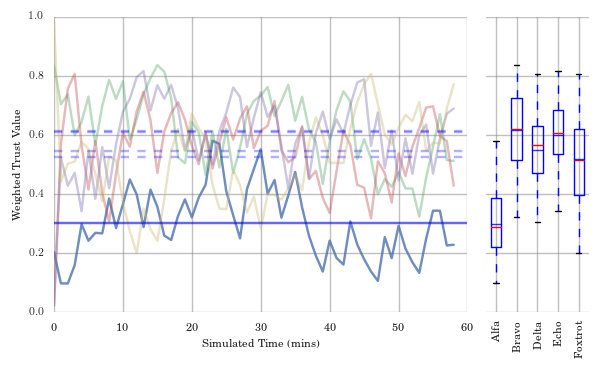
\includegraphics[width=\linewidth]{best_comms_run_SlowCoach}
  }
  \hfill
  \subfloat[Full Metric Trust Response\label{fig:full_slowcoach}]{%
    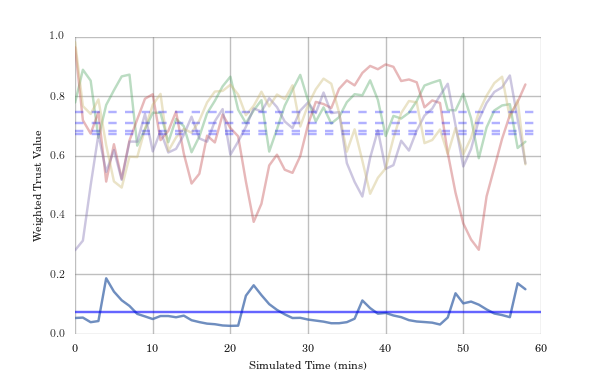
\includegraphics[width=\linewidth]{best_full_run_SlowCoach}
  }
  \caption{Trust Responses for SlowCoach using domain-optimised weights}
\end{figure}
%
\section{Results and Discussion}\label{sec:results}
Looking first at the arrived-at weighted metrics for the Multi-Domain ($X_{merge}$) case; shown in Table~\ref{tab:full_metric_correlations}; we see that the ``Physical'' Shadow misbehaviour is most heavily (and inversely) weighted to received signal strength; as is the SlowCoach physical behaviour. 
To demonstrate the operation of this method, it is useful to look at the difference between the trust response using a single-domain-optimised weighting and that of a multi-domain-optimised weighting; Fig.~\ref{fig:comms_slowcoach} shows the trust response using just $X_{comms}$, with a reasonable deviation in the highlighted node ($n_m$/Alfa), however in Fig.~\ref{fig:full_slowcoach}, where $X_{phys}$ is also included, this deviation is made extremely clear.

Table~\ref{tab:domain_deltas} summarises the average $\Delta T_{im}$ (specifically looking at the malicious node) and shows that on average, including all metrics improves the induced trust variation. 
It is useful to note however that it is not always ``better'' to include all metrics; $X_{phys}$ is better at differentiating SlowCoach behaviours, and $X_{comms}$ is slightly better at differentiating MPC and STS behaviours.
Some behaviours appear to be difficult to detect in any domain; Selfish Target Selection for example, with it's $\Delta T_{ix}$ making it significantly difficult to distinguish from environmental perturbations impacting trust assessment.



\section{Conclusion}
We have demonstrated that using metrics from across physical and communications domains to assess trust in UANs, this additional information can meaningfully improve induced ``deviation'' of misbehaviours trust responses to the point where they are more easily detectable and identifiable.
We have also demonstrated a purely analytical method for generating optimised metric weighting for MTFM using known behaviour training and Random Forest Regression.
In this case, we have naively included all possible metrics, and ``arbitrarily'' grouped those metrics into the domains they came from, but in interdependent systems such as UANs, these metrics may have significant cross-correlations and redundancies (for instance, Delay could be considered a function of node spacing which is also captured in INDD, which would also impact the received signal strength attained).
It may be the case that there exist more performant subsets of $X_{merge}$ that are significantly better at highlighting particular misbehaviours in isolation, and future work will investigate this very case; optimising subset-selection as we have optimised metric-weighting.

Further investigation is required to take this ``deviance'' and generate a dynamic run-time classifier based on this work. 
Particularly challenging will be the inclusion of collaborating malicious nodes and periodic misbehaviours; the current construction of $\Delta T_{ix}$ assumes that other nodes are fairly reporting their trust assessments, however if several nodes can sufficiently ``lie'' about how much they trust each other, the cohort based nature of MTFM could be exposed as a weakness.
Additionally, the scalability \& overhead challenges of applying this methodology to large numbers of small AUVs, such as pervasive sensor networks, is an open problem. 




% conference papers do not normally have an appendix


% use section* for acknowledgement
\section*{Acknowledgment}

The Authors would like to thank the DSTL/DGA UK/FR PhD Programme for their support during this project, as well as NATO CMRE for their advice and assistance.

\balance
\bibliographystyle{IEEEtran}
% argument is your BibTeX string definitions and bibliography database(s)
\bibliography{IEEEabrv,refs}

% that's all folks
\end{document}


% An example of a floating figure using the graphicx package.
% Note that \label must occur AFTER (or within) \caption.
% For figures, \caption should occur after the \includegraphics.
% Note that IEEEtran v1.7 and later has special internal code that
% is designed to preserve the operation of \label within \caption
% even when the captionsoff option is in effect. However, because
% of issues like this, it may be the safest practice to put all your
% \label just after \caption rather than within \caption{}.
%
% Reminder: the "draftcls" or "draftclsnofoot", not "draft", class
% option should be used if it is desired that the figures are to be
% displayed while in draft mode.
%
%\begin{figure}[!t]
%\centering
%\includegraphics[width=2.5in]{myfigure}
% where an .eps filename suffix will be assumed under latex, 
% and a .pdf suffix will be assumed for pdflatex; or what has been declared
% via \DeclareGraphicsExtensions.
%\caption{Simulation Results}
%\label{fig_sim}
%\end{figure}

% Note that IEEE typically puts floats only at the top, even when this
% results in a large percentage of a column being occupied by floats.


% An example of a double column floating figure using two subfigures.
% (The subfig.sty package must be loaded for this to work.)
% The subfigure \label commands are set within each subfloat command, the
% \label for the overall figure must come after \caption.
% \hfil must be used as a separator to get equal spacing.
% The subfigure.sty package works much the same way, except \subfigure is
% used instead of \subfloat.
%
%\begin{figure*}[!t]
%\centerline{\subfloat[Case I]\includegraphics[width=2.5in]{subfigcase1}%
%\label{fig_first_case}}
%\hfil
%\subfloat[Case II]{\includegraphics[width=2.5in]{subfigcase2}%
%\label{fig_second_case}}}
%\caption{Simulation results}
%\label{fig_sim}
%\end{figure*}
%
% Note that often IEEE papers with subfigures do not employ subfigure
% captions (using the optional argument to \subfloat), but instead will
% reference/describe all of them (a), (b), etc., within the main caption.


% An example of a floating table. Note that, for IEEE style tables, the 
% \caption command should come BEFORE the table. Table text will default to
% \footnotesize as IEEE normally uses this smaller font for tables.
% The \label must come after \caption as always.
%
%\begin{table}[!t]
%% increase table row spacing, adjust to taste
%\renewcommand{\arraystretch}{1.3}
% if using array.sty, it might be a good idea to tweak the value of
% \extrarowheight as needed to properly center the text within the cells
%\caption{An Example of a Table}
%\label{table_example}
%\centering
%% Some packages, such as MDW tools, offer better commands for making tables
%% than the plain LaTeX2e tabular which is used here.
%\begin{tabular}{|c||c|}
%\hline
%One & Two\\
%\hline
%Three & Four\\
%\hline
%\end{tabular}
%\end{table}


% Note that IEEE does not put floats in the very first column - or typically
% anywhere on the first page for that matter. Also, in-text middle ("here")
% positioning is not used. Most IEEE journals/conferences use top floats
% exclusively. Note that, LaTeX2e, unlike IEEE journals/conferences, places
% footnotes above bottom floats. This can be corrected via the \fnbelowfloat
% command of the stfloats package.


